\begin{frame}
  \frametitle{Keyboard Decoding}
  \framesubtitle{Scan Code Detection}
  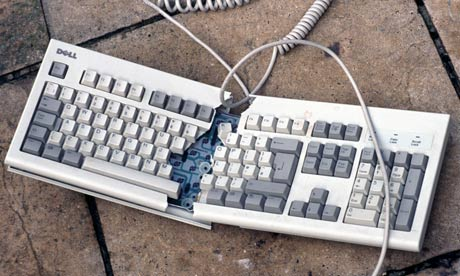
\includegraphics[scale=.6]{bkb.jpg}
\end{frame}
\begin{frame}
  \frametitle{Keyboard Decoding}
  \framesubtitle{Scan Code Detection}
  \begin{itemize}
  \item<1->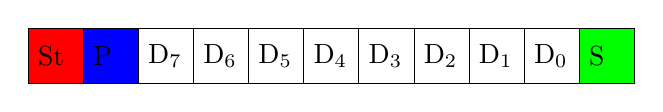
\begin{tikzpicture}[y=.7 cm, x=.7 cm]
    \draw(0,0) rectangle (11,1);
    \draw[fill=green] (10,0) rectangle (11,1);
    \draw[fill=blue] (1,0) rectangle (2,1);
    \draw[fill=red] (0,0) rectangle (1,1);
    \foreach \x in {1,...,10}
    \draw (\x, 0 ) -- ( \x, 1 );
    \draw (10,.5) node[anchor=west]{S};
    \draw (9,.5) node[anchor=west]{D$_0$};
    \draw (8,.5) node[anchor=west]{D$_1$};
    \draw (7,.5) node[anchor=west]{D$_2$};
    \draw (6,.5) node[anchor=west]{D$_3$};
    \draw (5,.5) node[anchor=west]{D$_4$};
    \draw (4,.5) node[anchor=west]{D$_5$};
    \draw (3,.5) node[anchor=west]{D$_6$};
    \draw (2,.5) node[anchor=west]{D$_7$};
    \draw (1,.5) node[anchor=west]{P};
    \draw (0,.5) node[anchor=west]{St};
  \end{tikzpicture}
  
  \item<2->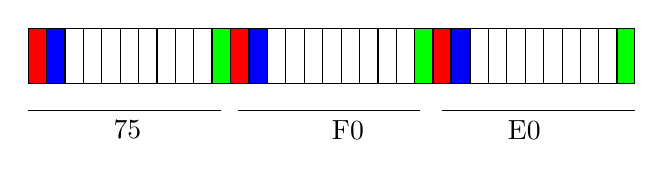
\begin{tikzpicture}[x=.7 cm, y=.7 cm]
    \draw(0,-2) rectangle (11,-1);
    \foreach \x in {3.333,7,10.666}
    \draw[fill=green] (\x,-2) rectangle (\x+.334,-1);
    \foreach \x in {.333,4,7.666}
    \draw[fill=blue] (\x,-2) rectangle (\x+.334,-1);
    \foreach \x in {0,3.666,7.333}
    \draw[fill=red] (\x,-2) rectangle (\x+.334,-1);
    \foreach \x in {0,.333,.667,...,11}
    \draw (\x, -2 ) -- ( \x, -1 );

    \draw (0,-2.5) -- (3.5,-2.5);
    \draw (1.8,-2.5) node[anchor=north]{75};
    \draw (3.8,-2.5) -- (7.1,-2.5);
    \draw (5.8,-2.5) node[anchor=north]{F0};
    \draw (7.5,-2.5) -- (11,-2.5);
    \draw (9,-2.5) node[anchor=north]{E0};
  
  \end{tikzpicture}
    
  \item<3->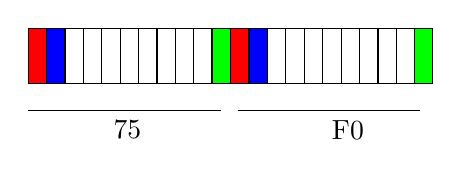
\begin{tikzpicture}[x=.7 cm, y=.7 cm]
    \draw(0,-2) rectangle (7.333,-1);

    \foreach \x in {3.333,7}
    \draw[fill=green] (\x,-2) rectangle (\x+.334,-1);
    \foreach \x in {.333,4}
    \draw[fill=blue] (\x,-2) rectangle (\x+.334,-1);
    \foreach \x in {0,3.666}
    \draw[fill=red] (\x,-2) rectangle (\x+.334,-1);
    \foreach \x in {0,.333,.667,...,7.333}
    \draw (\x, -2 ) -- ( \x, -1 );

    \draw (0,-2.5) -- (3.5,-2.5);
    \draw (1.8,-2.5) node[anchor=north]{75};
    \draw (3.8,-2.5) -- (7.1,-2.5);
    \draw (5.8,-2.5) node[anchor=north]{F0};
  
  \end{tikzpicture}

  \item<4->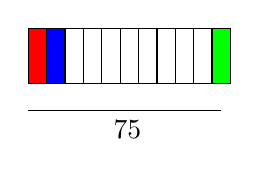
\begin{tikzpicture}[x=.7 cm, y=.7 cm]
    \draw(0,-2) rectangle (3.666,-1);

    \foreach \x in {3.333}
    \draw[fill=green] (\x,-2) rectangle (\x+.334,-1);
    \foreach \x in {.333}
    \draw[fill=blue] (\x,-2) rectangle (\x+.334,-1);
    \foreach \x in {0}
    \draw[fill=red] (\x,-2) rectangle (\x+.334,-1);
    \foreach \x in {0,.333,.667,...,3.666}
    \draw (\x, -2 ) -- ( \x, -1 );

    \draw (0,-2.5) -- (3.5,-2.5);
    \draw (1.8,-2.5) node[anchor=north]{75};
  
  \end{tikzpicture}
  \end{itemize}
  
\end{frame}

\begin{frame}
  \frametitle{Keyboard Decoding}
  \framesubtitle{Scan Code Detection}
  \begin{itemize}
    
  \item<1->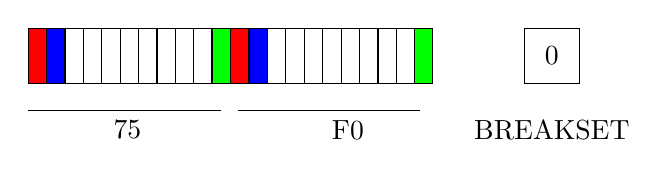
\begin{tikzpicture}[x=.7 cm, y=.7 cm]
    \draw(0,-2) rectangle (7.333,-1);

    \foreach \x in {3.333,7}
    \draw[fill=green] (\x,-2) rectangle (\x+.334,-1);
    \foreach \x in {.333,4}
    \draw[fill=blue] (\x,-2) rectangle (\x+.334,-1);
    \foreach \x in {0,3.666}
    \draw[fill=red] (\x,-2) rectangle (\x+.334,-1);
    \foreach \x in {0,.333,.667,...,7.333}
    \draw (\x, -2 ) -- ( \x, -1 );

    \draw (0,-2.5) -- (3.5,-2.5);
    \draw (1.8,-2.5) node[anchor=north]{75};
    \draw (3.8,-2.5) -- (7.1,-2.5);
    \draw (5.8,-2.5) node[anchor=north]{F0};

    \draw(9,-2) rectangle (10,-1);
    \draw(9.5,-1.5)  node{0};
    \draw (9.5,-2.5)  node[anchor=north]{BREAKSET};
  
  \end{tikzpicture}

  \item<2->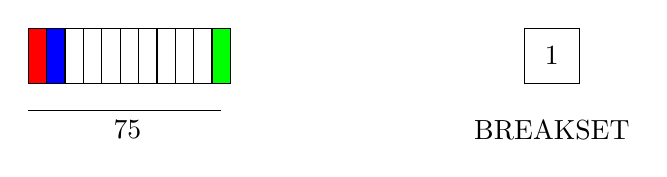
\begin{tikzpicture}[x=.7 cm, y=.7 cm]
    \draw(0,-2) rectangle (3.666,-1);

    \foreach \x in {3.333}
    \draw[fill=green] (\x,-2) rectangle (\x+.334,-1);
    \foreach \x in {.333}
    \draw[fill=blue] (\x,-2) rectangle (\x+.334,-1);
    \foreach \x in {0}
    \draw[fill=red] (\x,-2) rectangle (\x+.334,-1);
    \foreach \x in {0,.333,.667,...,3.666}
    \draw (\x, -2 ) -- ( \x, -1 );

    \draw (0,-2.5) -- (3.5,-2.5);
    \draw (1.8,-2.5) node[anchor=north]{75};

    \draw(9,-2) rectangle (10,-1);
    \draw(9.5,-1.5)  node{1};
    \draw (9.5,-2.5)  node[anchor=north]{BREAKSET};

  \end{tikzpicture}
  \item<3->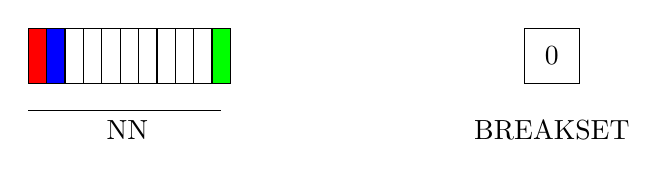
\begin{tikzpicture}[x=.7 cm, y=.7 cm]
    \draw(0,-2) rectangle (3.666,-1);

    \foreach \x in {3.333}
    \draw[fill=green] (\x,-2) rectangle (\x+.334,-1);
    \foreach \x in {.333}
    \draw[fill=blue] (\x,-2) rectangle (\x+.334,-1);
    \foreach \x in {0}
    \draw[fill=red] (\x,-2) rectangle (\x+.334,-1);
    \foreach \x in {0,.333,.667,...,3.666}
    \draw (\x, -2 ) -- ( \x, -1 );

    \draw (0,-2.5) -- (3.5,-2.5);
    \draw (1.8,-2.5) node[anchor=north]{NN};

    \draw(9,-2) rectangle (10,-1);
    \draw(9.5,-1.5)  node{0};
    \draw (9.5,-2.5)  node[anchor=north]{BREAKSET};

  \end{tikzpicture}
  \end{itemize}
  
\end{frame}
